\chapter{Arhitectura aplicației}

\section{Microservicii}

Aplicația adoptă paradigma arhitecturală a microserviciilor. Microserviciile presupun segmentarea unei aplicații într-o suită de servicii specializate, independente, ce comunică prin protocoale light-weight. Pentru comunicare am ales cea mai populară formă, API-urile bazate pe HTTP. Unul din avantajele principale ale acestei arhitecturi este decuplarea serviciilor implicate. Eșecul unui serviciu nu afectează întreaga aplicație, astfel încât problemele se manifestă izolat și sunt mai ușor de controlat. Un alt motiv pentru care am considerat că această arhitectură este potrivită aplicației este versatilitatea permisă în alegerea tehnologiilor și a limbajelor de programare\cite{building_microservices}.  Într-o aplicație monolit, această libertate nu ar fi fost posibilă.

 \begin{figure}[ht]
	\centering
 	 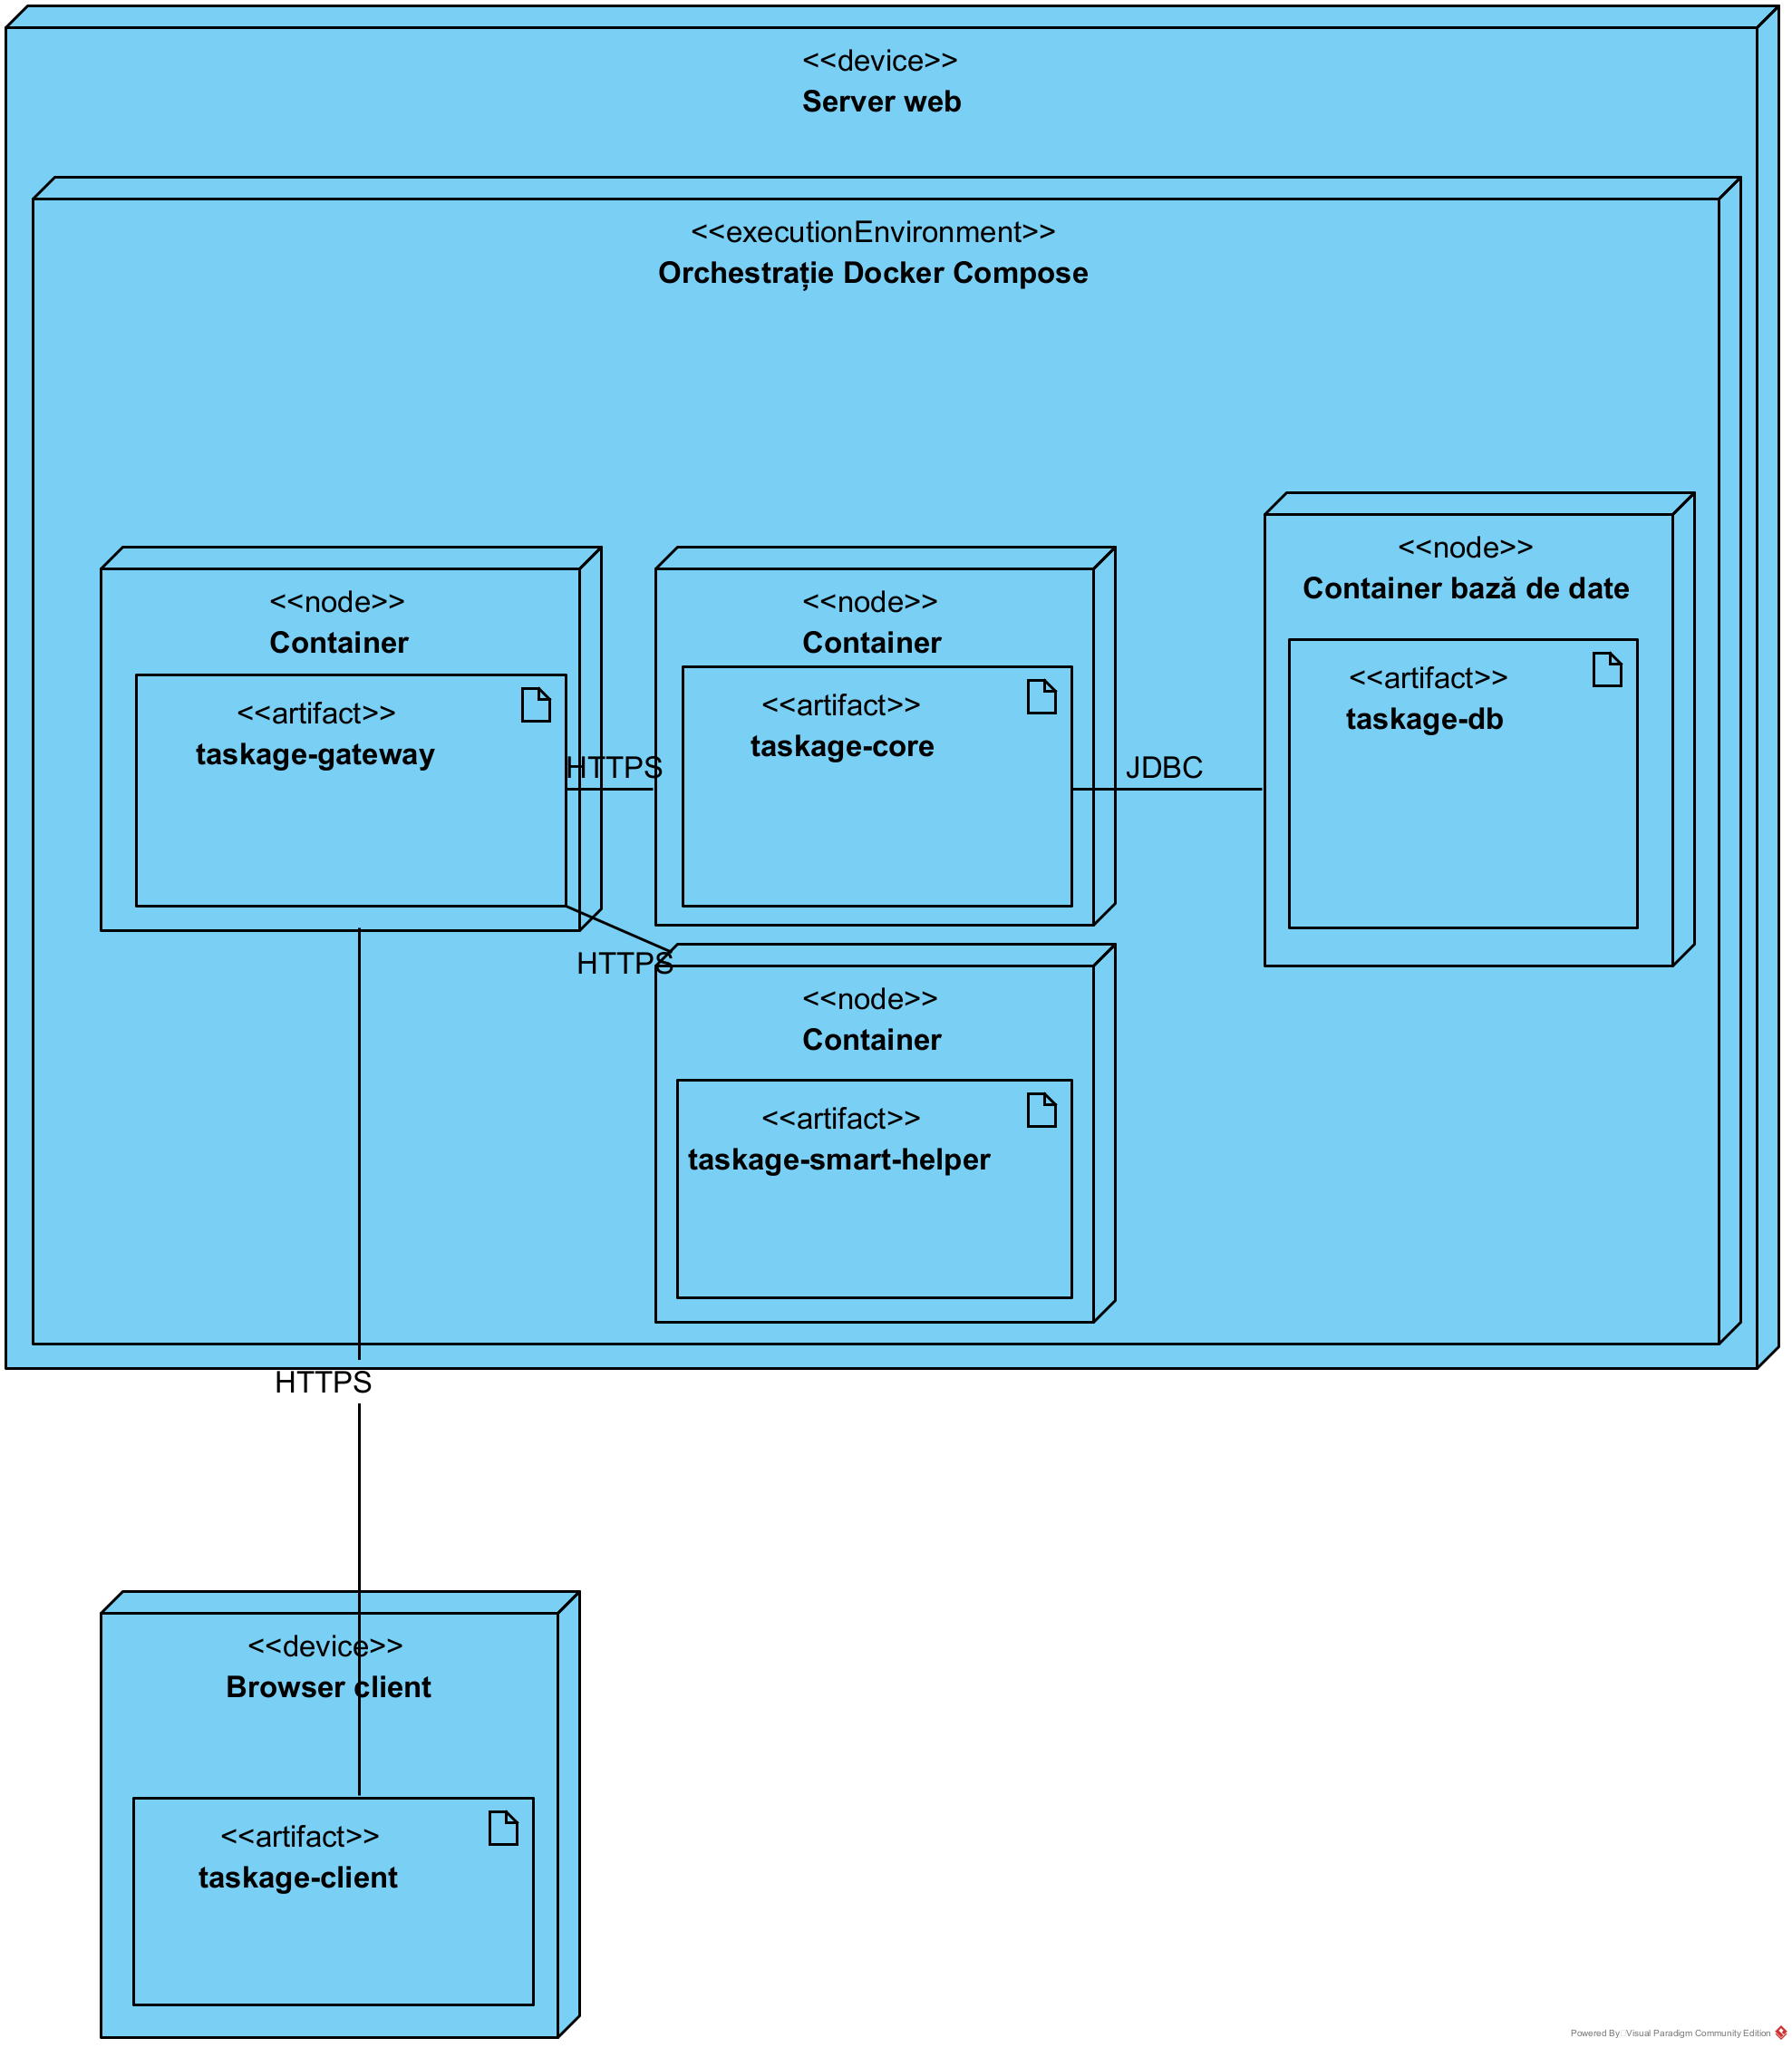
\includegraphics[width=\linewidth]{deployment-diagram.png}
	\caption{Diagrama de desfășurare}
	\label{fig:deployment-diagram}
 \end{figure}

Figura \ref{fig:deployment-diagram} ilustrează natura modulară a aplicației și integrarea diferitelor microservicii. Pe partea de front-end, artefactul aplicației React Taskage-Client rulează în browser-ul web al utilizatorului prin codul transpilat din TSX în JS. Acesta comunică cu serverul prin apeluri HTTP, utilizând componenta Spring Cloud Taskage-Gateway ca punct de intrare către functionalitățile back-end. Acest punct de intrare redirecționează apelurile spre componenta potrivită, pe baza configurărilor indicate în fișierul application.yml. Un gateway este un intermediar rafinat, oferind și posibilități de service discovery și load balancing. Apelul este trimis mai departe prin HTTP, iar conexiunile la baza de date sunt făcute prin JDBC pentru componenta Taskage-Core, respectiv toolkit-ul Flask-SQLAlchemy pentru componenta Taskage-Helper. Scopul componentei Taskage-Core este reprezentat de operațiile centrale aplicației, în principal CRUD, în timp ce componenta Taskage-Helper nu face decât operații de citire asupra bazei de date, scopul ei fiind analiza datelor stocate.

\section{Taskage-Gateway}

Un API gateway servește, în general, drept singurul punct de contact dintre aplicații externe sau interfețe utilizator și back-end-uri și este specific arhitecturii bazate pe microservicii. Aceasta gestionează cererile HTTP ce ajung la ea și le redirecționează, comportându-se ca un „om de mijloc” (middleman) între interfață și logica de afaceri sau sursa de date.  Cunoscut și sub denumirea de „reverse proxy”, poate analiza cererile primite și, în funcție de cale, headers și parametrii și poate decide încotro le va redirecționa.

Mai mult, API gateway-ul poate să gestioneze în mod eficient volumului de cereri ce ajunge către fiecare replică a unui serviciu, în cadrul unei arhitecturi bazată pe microservicii, pe baza unui algoritm de load balancing precum Round Robin, Least Connections, sau Weighted Distribution.

Există multe soluții pentru API gateway-uri ce necesită configurare minimă, ce vin de la toți giganții industriei Cloud (Google - Cloud Endpoints, Amazon - Amazon API Gateway, Microsoft - Azure API Gateway), însă există și soluții open-source, precum Apache APISIX API Gateway. În cadrul proiectului Taskage, este folosit Spring Cloud Gateway, fiind ușor de utilizat și configurat, necesitând în principal dependințe de Maven și un fișier de configurări, fișier de tip resursă, „application.yml”(figura \ref{fig:yaml}), în cadrul căruia sunt definite regulile de rutare aferente, sub secțiunea „cloud.gateway”.

Putem observa diverse componente de configurare: secțiunea routes prezintă configurările aferente rutării cererilor primite de către API gateway, sub care vine fiecare rută în parte, alături de URI-ul ei, și configurări adiționale, precum modelul căii cererii ce va intra pe această rută. În plus, se poate observa și secțiunea filters, sub care Spring Cloud Gateway îți permite să definești o gamă largă de filtre ce urmează să fie aplicate cererii, precum adăugarea de circuit breakere, rescrierea căii specifice sau prefixarea/sufixarea acesteia, sau, cum este cazul în configurarea prezentată, adăugarea unui header cu o valoare specifică pentru a valida că cererea a trecut întâi prin API Gateway și nu a fost făcută în mod direct endpoint-ului REST.

\begin{figure}[H]
	\begin{lstlisting}[frame=single, style=yaml]
  cloud:
    gateway:
      routes:
        - id: core
          uri: http://127.0.0.1:8080
          predicates:
            - Path=/**
          filters:
            - AddRequestHeader=X-XSRF-Token, ValidToken
      globalcors:
        cors-configurations:
          "[/**]":
            allowed-origins:
              - http://localhost:3000
            allowedMethods: "GET, POST, PUT, DELETE, OPTIONS"
            allowedHeaders: "Origin, X-Requested-With, Content-Type, Accept, Content-Length, TOKEN, Authorization"
            allowCredentials: true
            maxAge: 3600
	\end{lstlisting}
	\caption{application.yml}
	\label{fig:yaml}
\end{figure}

În plus, se pot face și configurări în ceea ce privește „cross-origin request forgery”, ce se pot configura per rută și vizează parametrii precum origini permise, metode HTTP permise și headere permise, ca măsură de securitate.

\section{Taskage-Core}

 \begin{figure}[ht]
	\centering
 	 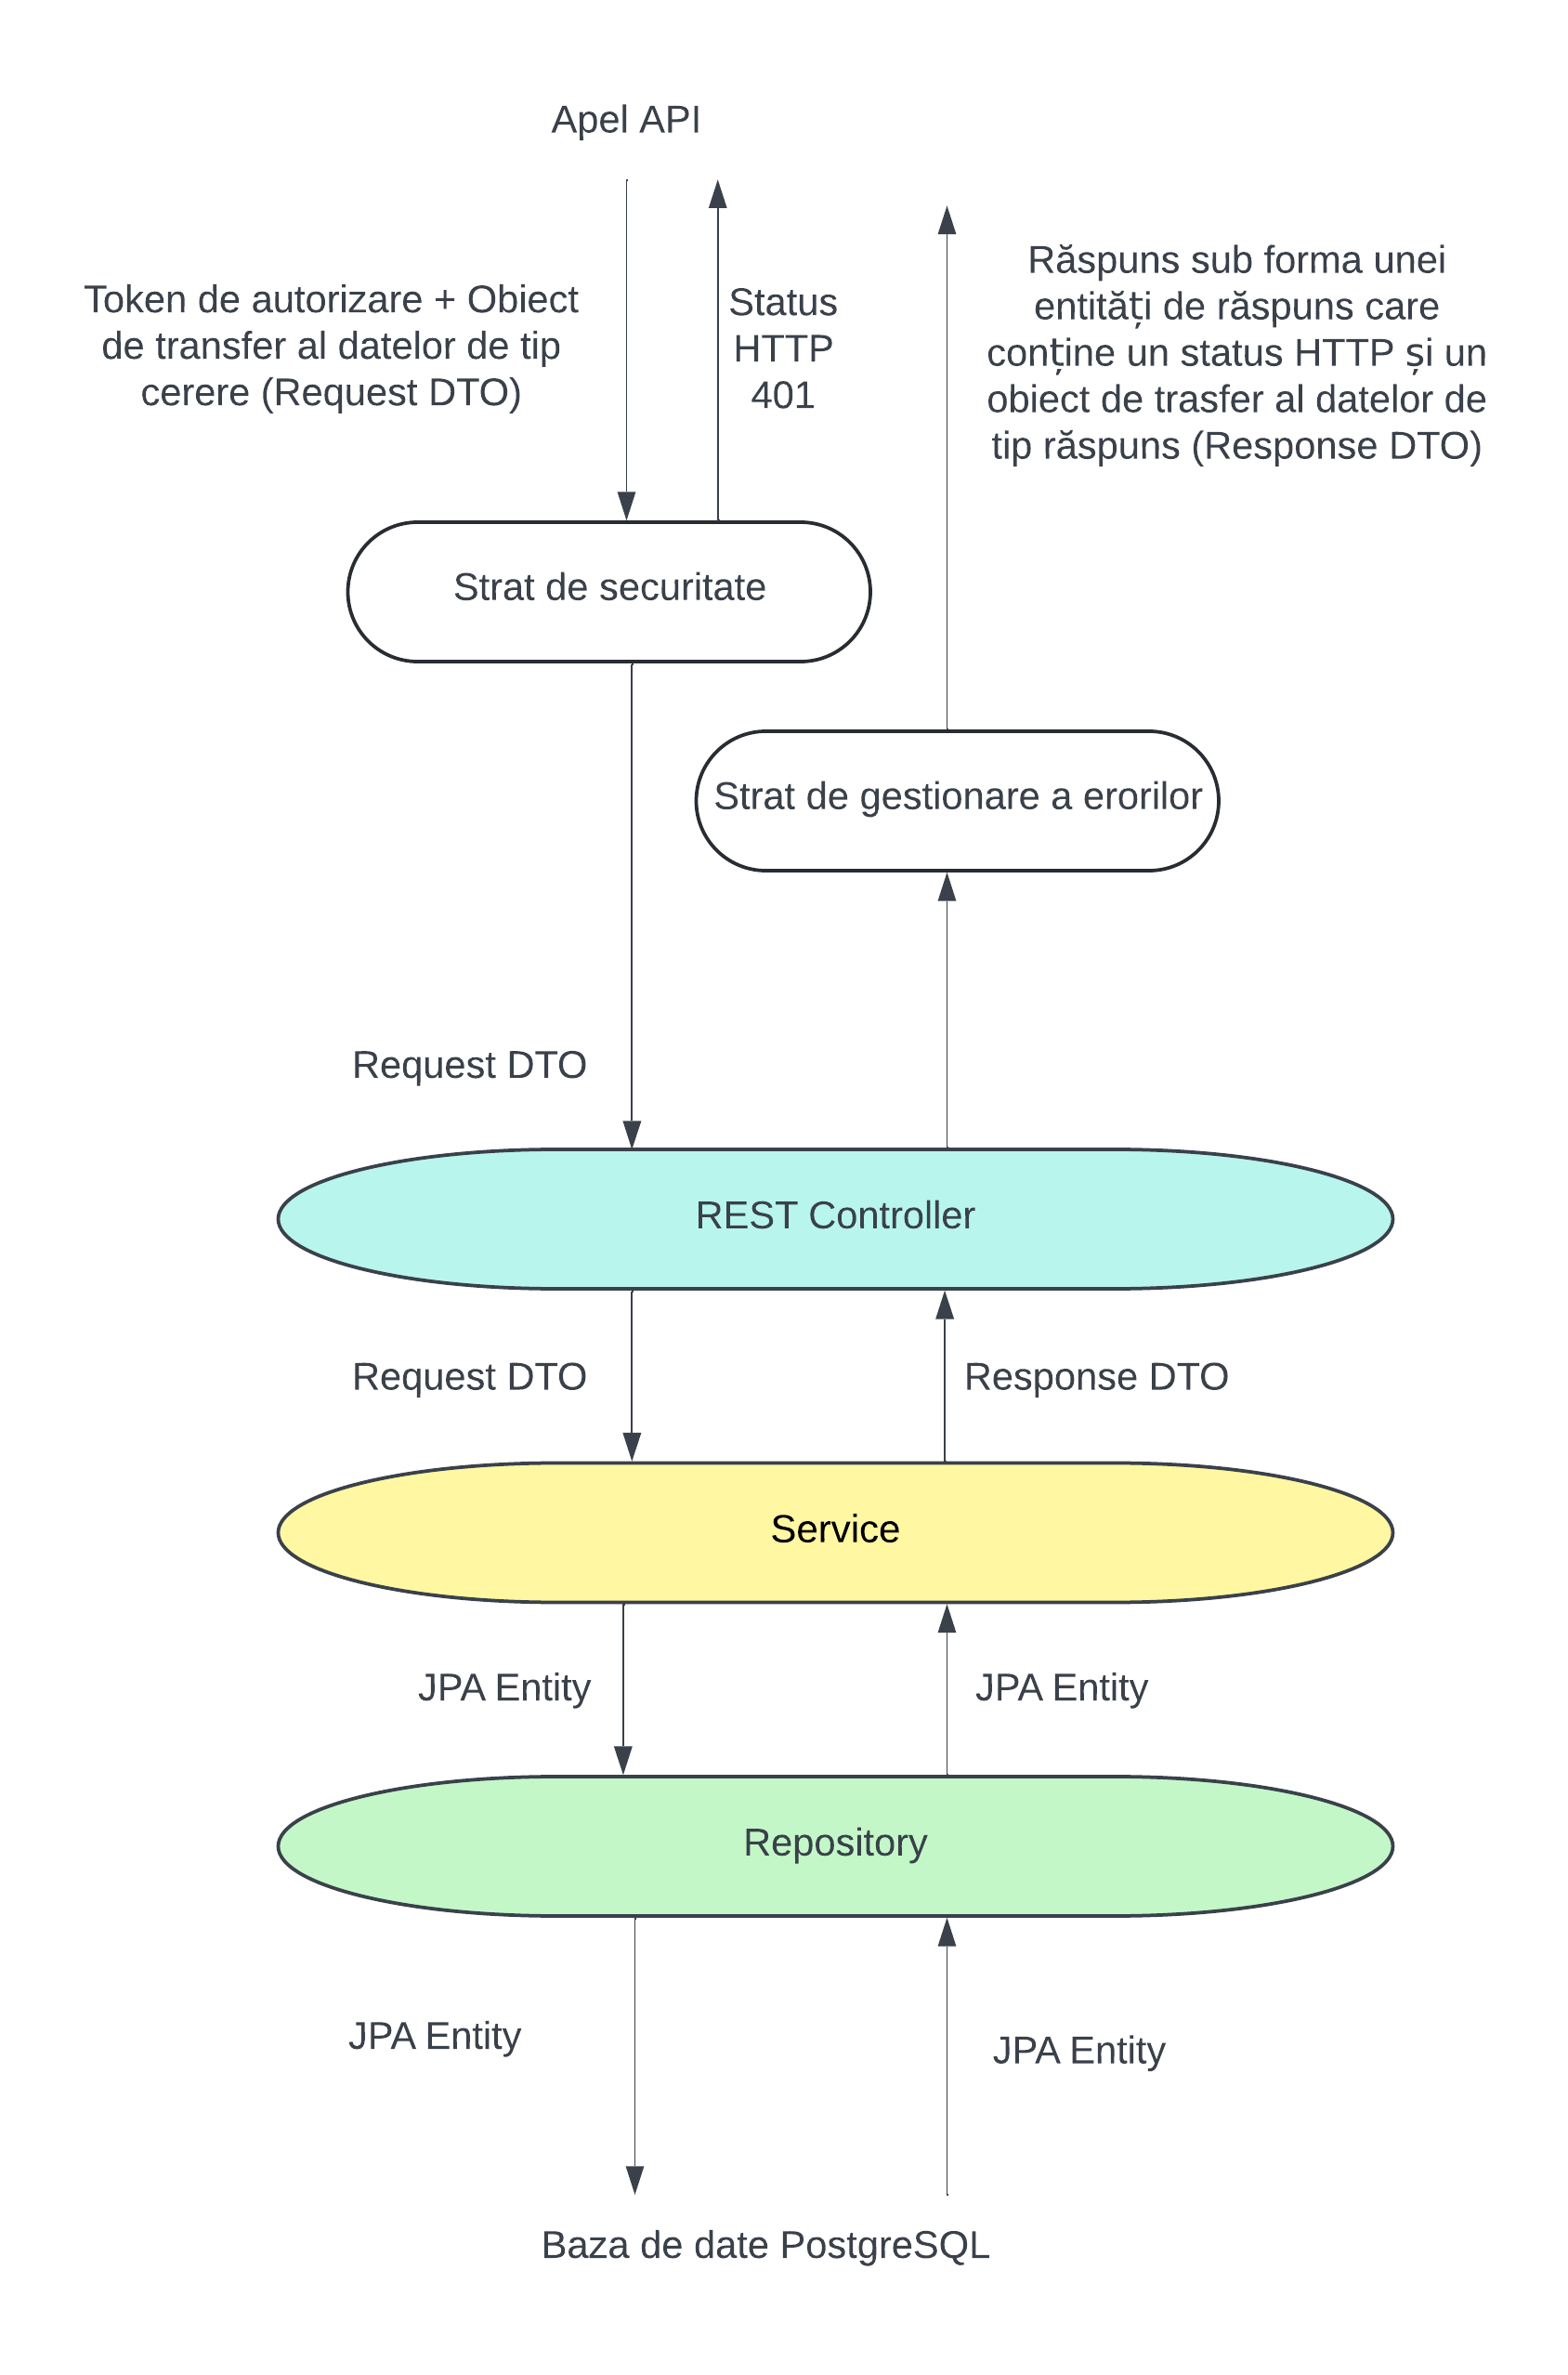
\includegraphics[width=0.6\linewidth]{controller-service-repository-flow.png}
	\caption{Fluxul datelor în componenta core}
	\label{controller-service-repository-flow}
 \end{figure}

Componenta care se ocupă cu funcționalitățile cele mai de bază ale aplicației este Taskage-Core. Aici se realizează operațiile CRUD asupra entităților și se gestionează cererile uzuale ale platformei. Structura componentei urmează patternul Controller-Service-Repository, popular în aplicațiile Spring Boot. Acest model de structurare a proiectului urmărește separarea sarcinilor unui sistem mare în părți mai ușor de manevrat. Fluxul datelor, reprezentat în figura \ref{controller-service-repository-flow}, este controlat, iar fiecare strat are un scop bine definit. 

Apelurile HTTP conțin un JWT token în header și trec prin filtrul de autorizare, implementat cu ajutorul Spring Securit. Dacă tokenul este aprobat ca fiind valabil și având criptat rolul corespunzător, apelul ajunge la end-point-ul asociat din controller. Altfel, aplicația intoarce un răspuns cu status HTTP 401(Unauthorized). Controllerele constituie API-ul aplicației și ca au ca unic scop expunerea unor funcționalități către agenți externi. Datele sunt primite sub forma unui obiect de transfer al datelor(Request DTO), care nu se traduce într-o entitate a bazei de date, fiind doar un mod de transmitere a informației între microservicii. Aceste DTO-uri trebuie de asemenea să respecte validările impuse câmpurilor prin Jakarta Validation.

Dacă DTO-ul a fost validat, acesta este trimis mai departe pentru procesare în zona cu logica de afaceri a aplicației, și anume serviciile. Serviciile procesează informația și eventual o mapează ca entități JPA spre a o transmite mai departe depozitelor(repositories). Depozitele reprezintă stratul de acces al datelor și se ocupă cu toate interacțiunile cu baza de date. Dacă totul se realizează cu succes, se va returna o entitate de răspuns cu statusul HTTP 200, eventual conținând un Response DTO cu datele cerute. Dacă se aruncă vreo excepție, aceasta va fi prinsă de clasa care se ocupă cu gestiunea erorilor la nivel global, GlobalExceptionHandler, și se va trimite înapoi un răspuns sugestiv.

\section{Taskage-DB}

Schema bazei de date este concepută pentru a stoca toate informațiile necesare gestionării unui proiect și generării de sugestii relevante. Urmărind o delimitare clară a responsabilităților, am identificat următoarele entități și relații(figura \ref{erd}):

 \begin{figure}[H]
	\centering
 	 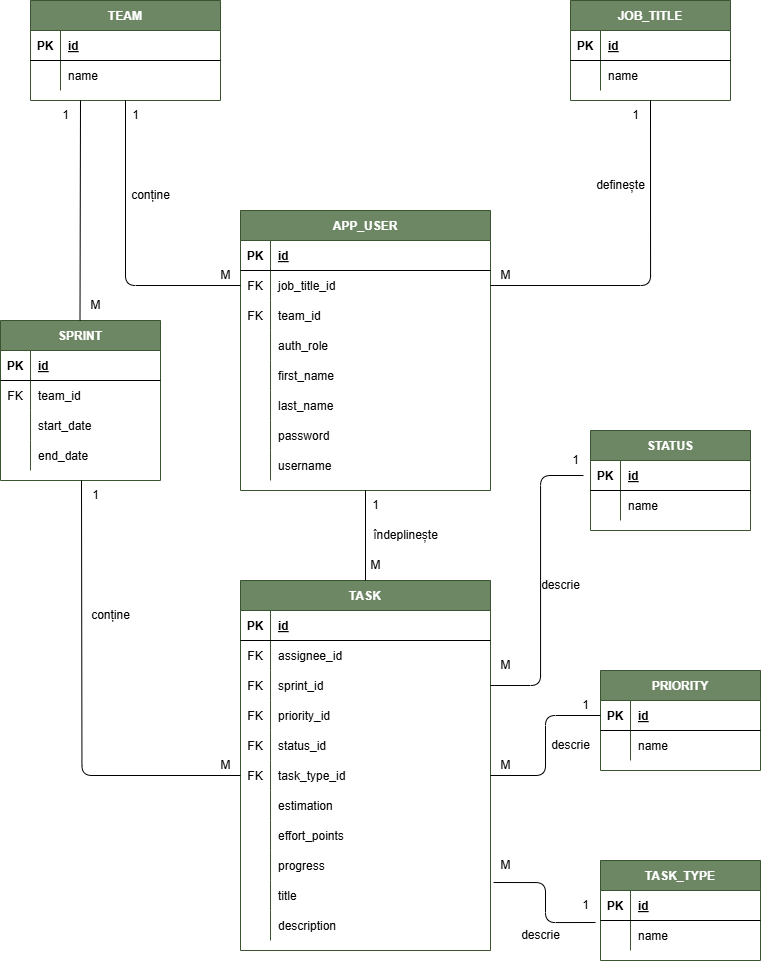
\includegraphics[width=1\linewidth]{ERD.png}
	\caption{Diagrama entitate-relație}
	\label{erd}
 \end{figure}

\begin{enumerate}
 	 \item \textbf{Team}(Echipă):
\begin{itemize}
\item[--] Atribute: id (PK), name
\item[--] Relații: App user(1:M), Sprint(1:M)
\item[--] Descriere: Reprezintă o echipă care lucrează la un proiect. Fiecare echipă are un id și un nume unice și o listă de utilizatori și sprinturi asociată.
\end{itemize}
	\item \textbf{Job title}(Poziție):
\begin{itemize}
\item[--] Atribute: id (PK), name
\item[--] Relații: App user(1:M)
\item[--] Descriere: Definește rolurile care se pot atribui în cadrul echipei. Fiecare rol poate fi asociat mai multor utilizatori. Fiecare înscriere a unui utilizator permite adăugarea unui nou rol.
\end{itemize}
	\item \textbf{App user}(Utilizator):
\begin{itemize}
\item[--] Atribute: id (PK), job_title_id (FK), team_id (FK), auth_role, first_name, last_name, password, username
\item[--] Relații: Team(M:1), Job title(M:1), Task(1:M)
\item[--] Descriere: Reprezintă un utilizator înregistrat în sistem de către administrator. Administratorul este adăugat o dată cu crearea bazei de date, făcând parte din „seed data”. Fiecare utilizator este asociat unei echipe, unui rol și se poate asocia mai multor sarcini de lucru.
\end{itemize}
	\item \textbf{Sprint}(Sprint):
\begin{itemize}
\item[--] Atribute: id (PK), team_id (FK), start_date, end_date
\item[--] Relații: Task(1:M), Team(M:1)
\item[--] Descriere: Reprezintă un sprint(unitate de timp în care membrii se angajează să livreze un set de funcționalități) din cadrul unui proiect. Fiecare sprint este legat de o echipă și poate conține mai multe sarcini de lucru.
\end{itemize}
	\item \textbf{Task}(Sarcină de lucru): 
\begin{itemize}
\item[--] Atribute: id (PK), assignee_id (FK), sprint_id (FK), priority_id (FK), status_id (FK), task_type_id (FK), estimation, effort_points, progress, title, description
\item[--] Relații: App user(M:1), Sprint(M:1), Priority(M:1), Status(M:1), Task type(M:1) 
\item[--] Descriere: Entitatea centrală, reprezentând sarcinile de lucru. Fiecare sarcină de lucru este asignată unui utilizator, unui sprint, și este descrisă de un status, o prioritate și un tip de task.
\end{itemize}
	\item \textbf{Status}(Status): 
\begin{itemize}
\item[--] Atribute: id (PK), name
\item[--] Relații: Task(1:M)
\item[--] Descriere: Definește statusurile posibile unei sarcini de lucru(tabelă dicționar).
\end{itemize}
	\item \textbf{Priority}(Prioritate): 
\begin{itemize}
\item[--] Atribute: id (PK), name
\item[--] Relații: Task(1:M)
\item[--] Descriere: Definește prioritățile posibile unei sarcini de lucru(tabelă dicționar).
\end{itemize}
	\item \textbf{Task type}(Tip de sarcină de lucru): 
\begin{itemize}
\item[--] Atribute: id (PK), name
\item[--] Relații: Task(1:M)
\item[--] Descriere: Definește tipurile posibile unei sarcini de lucru(tabelă dicționar).
\end{itemize}
\end{enumerate}

Fiecare tabel este normalizat pentru a preveni redundanța, iar multitudinea de tabele dicționar susține flexibilitatea și scalabilitatea. Varianta alternativă, salvarea dicționarelor în back-end prin intermediul tipului de date „enum”, presupune re-compilarea și re-deployerea aplicației pentru orice mică schimbare a cerințelor, în timp ce o modificare în baza de date este mult mai puțin costisitoare. De asemenea, construcția unui „enum” pentru etichetele folosite în interfața pentru utilizatori ar implica duplicarea datelor, ele trebuind declarate și în back-end și în front-end. În plus, legăturile definite de foreign keys asigură integritatea datelor, prevenind apariția de valori invalide.

Tabela „app_users” are câmpul special „auth_role” care poate lua una din valorile „ROLE_BASIC”(asociat membrilor normali ai unei echipe), „ROLE_MANAGER”(asociat managerilor echipelor) și „ROLE_ADMIN”(asociat administratorului paginii), urmând formatul înțeles de Spring Security. Speciale mai sunt tabelele de tip dicționar „priorities” și „statuses”, care nu implementează operații CRUD, ci servesc la stocarea unor date care altfel ar fi fost stocate în structuri de tip enum. Această alegere ajută la organizarea eficientă a codului și permite manevrarea mai ușoară a valorilor, putând fi chiar și actualizate la runtime.

\section{Taskage-Client}

Componenta care constituie front-end-ul aplicației este Taskage-Client. Aceasta este un proiect React care folosește MobX pentru gestionarea stării. Una din provocările principale la construcția unui proiect în React este lipsa de structură inerentă tehnologiei. Proiectele React nu au o structură de fișiere și un flux de date bine-definite, acestea rămânând responsabilitatea dezvoltatorului. Cele două mari abordări pentru structurarea aplicației sunt: abordarea orientată pe cateogorie și abordarea orientată spre funcționalitate. Prima variantă este mai puțin scalabilă, organizând fișierele după tipul lor(componente, pagini, modele) în timp ce a doua abordare rafinează mai departe structura, sortând componentele în funcție de funcționalitatea efectivă pe care o implementează. Din acest motiv am ales cea de-a doua alternativă.

 \begin{figure}[ht]
	\centering
 	 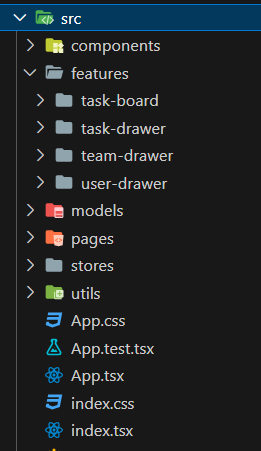
\includegraphics[width=0.3\linewidth]{FE-folder-structure.png}
	\caption{Structura de fișiere a aplicației React}
	\label{FE-folder-structure}
 \end{figure}

Deși front-end-ul reprezintă un SPA(Single Page Application), încărcarea paginilor se face pe baza rutelor pentru eficiență. Rutele sunt atât publice, cât și private. Cele private se pot accesa pe baza unor criterii precum tipul utilizatorului, iar în cazul lipsei privilegiilor de acces, acestea vor redirecționa utlizatorul către o pagină cu un mesaj sugestiv. Rutele servesc pagini, implementate în folderul „pages”, iar paginile randează diverse componente care, daca au logică complexă, sunt plasate într-un folder cu nume sugestiv funcționalității de care țin, în folderul „features”. Folderul „components” este rezervat pentru componente reutilizabile, generice. Stocarea datelor necesare în componente aflate la distanță mare pe ierarhia din DOM se face in „stores”, concept specific MobX. Tot aici se fac si apelurile către server și gestionarea datelor utilizatorului spre setarea corespunzătoare a tokenului în header-ul cererilor.

\section{Taskage-Helper}

Componenta care se ocupă cu analiza datelor stocate este Taskage-Helper. Aceasta este dezvoltată folosind Flask și comunică prin apeluri de API cu front-end-ul. Se observă faptul că este decuplată de celălalt serviciu de back-end, dezvoltarea sa putându-se realiza independent. Structura urmează o variantă adaptată a Controller-Service-Repository, în care filele sunt grupate în controllers, services și models, deoarece am ajuns la concluzia ca interacțiunea cu baza de date este prea simplă pentru a adăuga stratul de persistență. Operațiile de citire sunt executate direct din serviciile care au nevoie de datele respective. Terminologia Flask este destul de diferită de cea Spring Boot, astfel încât controllerele sunt numite „Blueprints” iar clasele care reprezintă entități ale bazei de date moștenesc clasa de bază „Model”.

Diagrama de secvență din figura \ref{sequence-diagram} reprezintă o expunere vizuală a interacțiunii dintre diferite componente ale aplicației, ca răspuns la acțiunea utilizatorului de click al butonului de cerere a sugestiei. Se observă clar fluxul controlat al informației într-o manieră abstractizată.

 \begin{figure}[H]
	\centering
 	 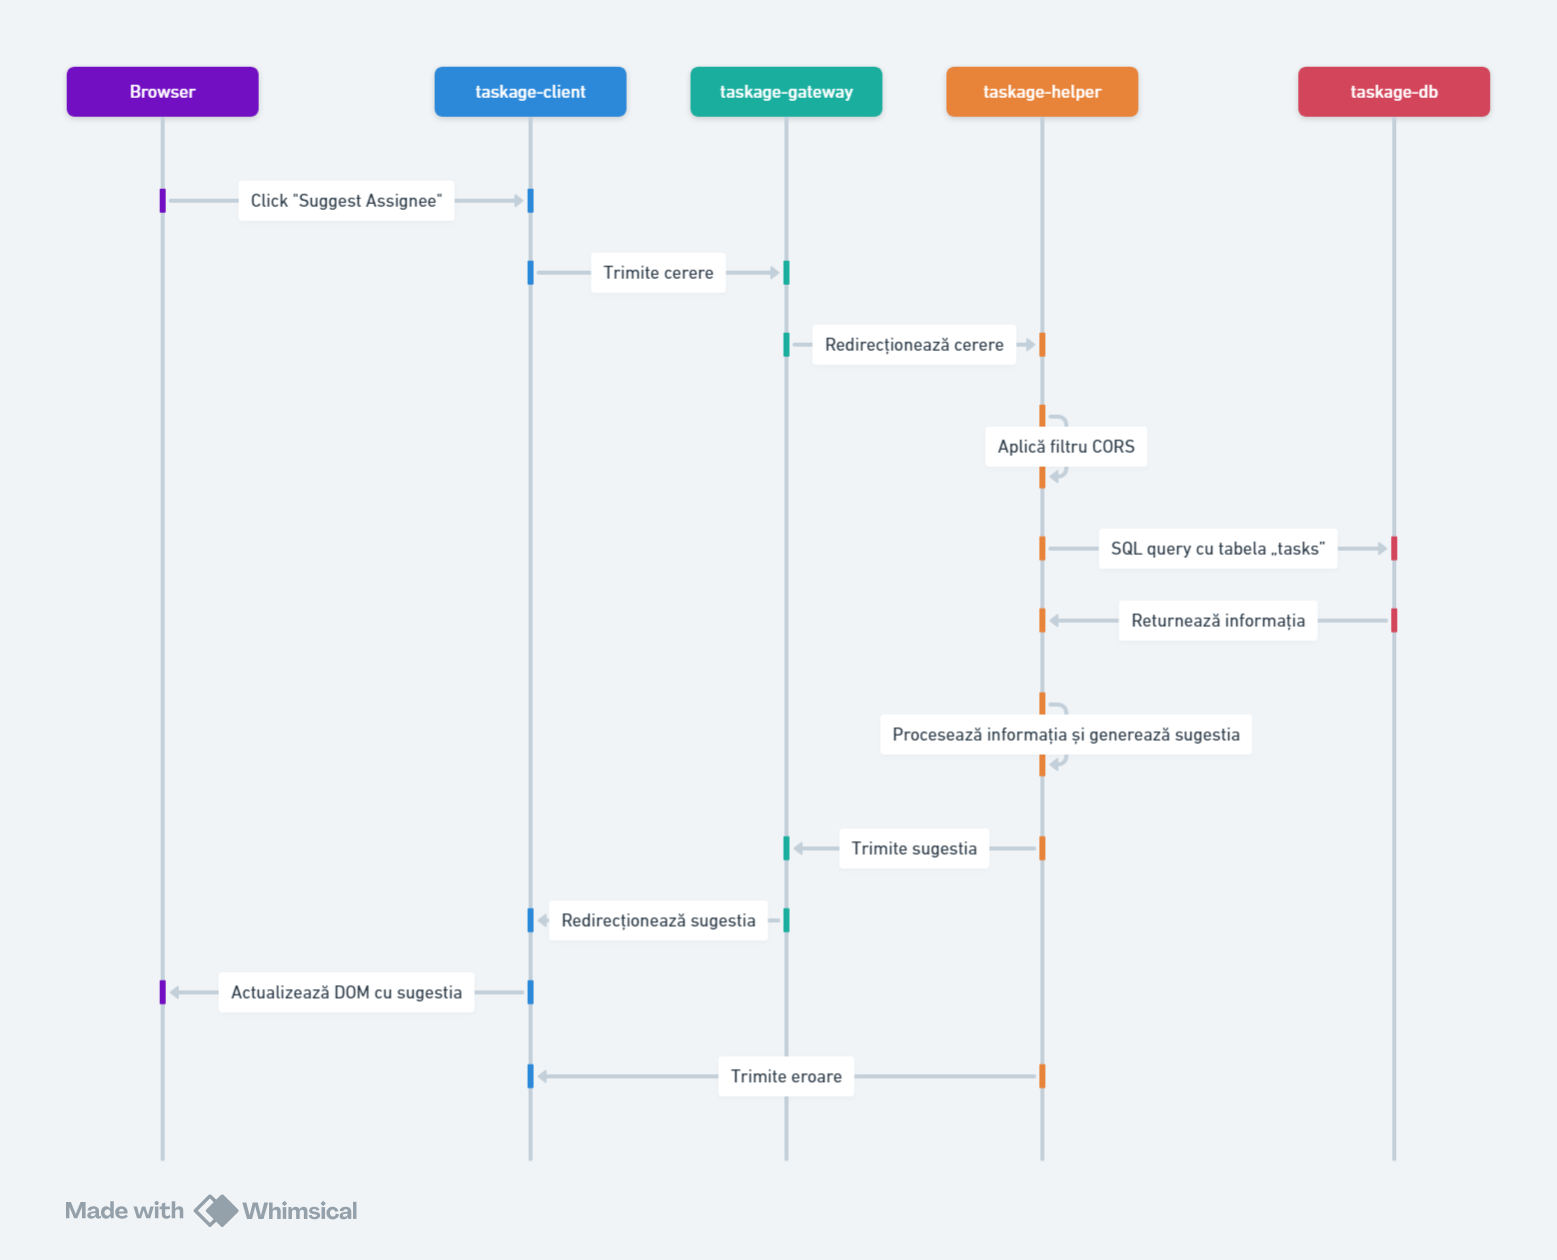
\includegraphics[width=1\linewidth]{sequence-diagram.png}
	\caption{Diagrama de secvență a Taskage-Helper}
	\label{sequence-diagram}
 \end{figure}